%%%%%%%%%%%%%%%%%%%%%%%%%%%%%%%%%%%%%%%%%
% https://www.overleaf.com/4390298fyrgbt#/13091088/
% a0poster Landscape Poster
% LaTeX Template
% Version 1.0 (22/06/13)
%
% The a0poster class was created by:
% Gerlinde Kettl and Matthias Weiser (tex@kettl.de)
% 
% This template has been downloaded from:
% http://www.LaTeXTemplates.com
%
% License:
% CC BY-NC-SA 3.0 (http://creativecommons.org/licenses/by-nc-sa/3.0/)
%
%%%%%%%%%%%%%%%%%%%%%%%%%%%%%%%%%%%%%%%%%
%----------------------------------------------------------------------------------------
%	PACKAGES AND OTHER DOCUMENT CONFIGURATIONS
%---------------------------------------------------------------------------------------

\documentclass[a222,landscape]{a0poster}

\usepackage{multicol} % This is so we can have multiple columns of text side-by-side
\columnsep=100pt % This is the amount of white space between the columns in the poster
\columnseprule=3pt % This is the thickness of the black line between the columns in the poster

\usepackage[svgnames, table]{xcolor} % Specify colors by their 'svgnames', for a full list of all colors available see here: http://www.latextemplates.com/svgnames-colors

\usepackage{times} % Use the times font
%\usepackage{palatino} % Uncomment to use the Palatino font

%\usepackage[scale=1.24]{beamerposter} % Use the beamerposter package for laying out the poster
%\setlength{\paperwidth}{48in} % A0 width: 46.8in
%\setlength{\paperheight}{36in} % A0 height: 33.1in

\usepackage{graphicx} % Required for including images
\graphicspath{{figures/}} % Location of the graphics files
\usepackage{booktabs} % Top and bottom rules for table
\usepackage[font=small,labelfont=bf]{caption} % Required for specifying captions to tables and figures
\usepackage{amsfonts, amsmath, amsthm, amssymb} % For math fonts, symbols and environments
\usepackage{wrapfig} % Allows wrapping text around tables and figures
\begin{document}


%----------------------------------------------------------------------------------------
%	POSTER HEADER 
%----------------------------------------------------------------------------------------

% The header is divided into three boxes:
% The first is 55% wide and houses the title, subtitle, names and university/organization
% The second is 25% wide and houses information
% The third is 19% wide and houses a logo for your university/organization or a photo of you
% The widths of these boxes can be easily edited to accommodate your content as you see fit

\begin{minipage}[b]{0.75\linewidth}
\veryHuge \color{NavyBlue} \textbf{An Exploratory Data Analysis of Uber Based on Twitter} \color{Black}\\ % Title
% \Huge\textit{Presented}\\[0.5 cm] % Subtitle
\huge \textbf{Presented by Aksam Ahmad, Siyao Chang, Fengshi Niu, Chenyu Wang, and Xinyue Zhou}\\
% \huge University and Department Name\\
\end{minipage}
\begin{minipage}[b]{0.25\linewidth}
\raggedleft
\includegraphics[width=0.5\linewidth]{../figures/Poster_OldNewLogo.png}
\end{minipage}


\vspace{0.5 cm} % A bit of extra whitespace between the header and poster content

%----------------------------------------------------------------------------------------

\begin{multicols}{4} % This is how many columns your poster will be broken into, a poster with many figures may benefit from less columns whereas a text-heavy poster benefits from more


\color{Navy} % Navy color for the abstract

\color{DarkRed} % SaddleBrown color for the introduction

\section*{Introduction}
% added by fengshi 02-20 2:13 
In our analysis, we are look at tweets about Uber as a way of understanding the public’s mindset about Uber and its services. Our exploratory analysis begins with answering certain questions, such as when, where and what do people about Uber. Along the way, we do further analysis on the negative tweets. Finally, tweets pertaining to surge pricing, the key pricing strategy of the firm, and tweets pertaining to its new logo are decomposed further.

% The goal is to help the firm quickly catch customer’s and driver’s real-time interest related to firm so as to take actions accordingly. 

\color{DarkSlateGray} % DarkSlateGray color for the rest of the content

\section*{Data Collection and Mining}

\begin{itemize}
   \item English tweets with containing \#Uber from January 20, 2016 to February 13, 2016
   \item Subset tweets with a UTC-offset value and converted to local time
   \item Tokenized tweets and removed stop and auxiliary words
\end{itemize}


% OLD - To be removed - Aksam
% We acquired data by using the search tweet function of twitter API. Our data include all tweets in English with \#uber from January 20 to February 13, 2016.
% For pre-processing, we subset for all the tweets with a utc-offset value since we are only able to convert the utc time to local time for the tweets with utc-offset values. Then, we tokenized the tweets and took out all the stop words and auxiliary words.



%----------------------------------------------------------------------------------------
%	MATERIALS AND METHODS
%----------------------------------------------------------------------------------------

\section*{Most Frequently Tweeted Words With Uber}

\begin{center}\vspace{1cm}

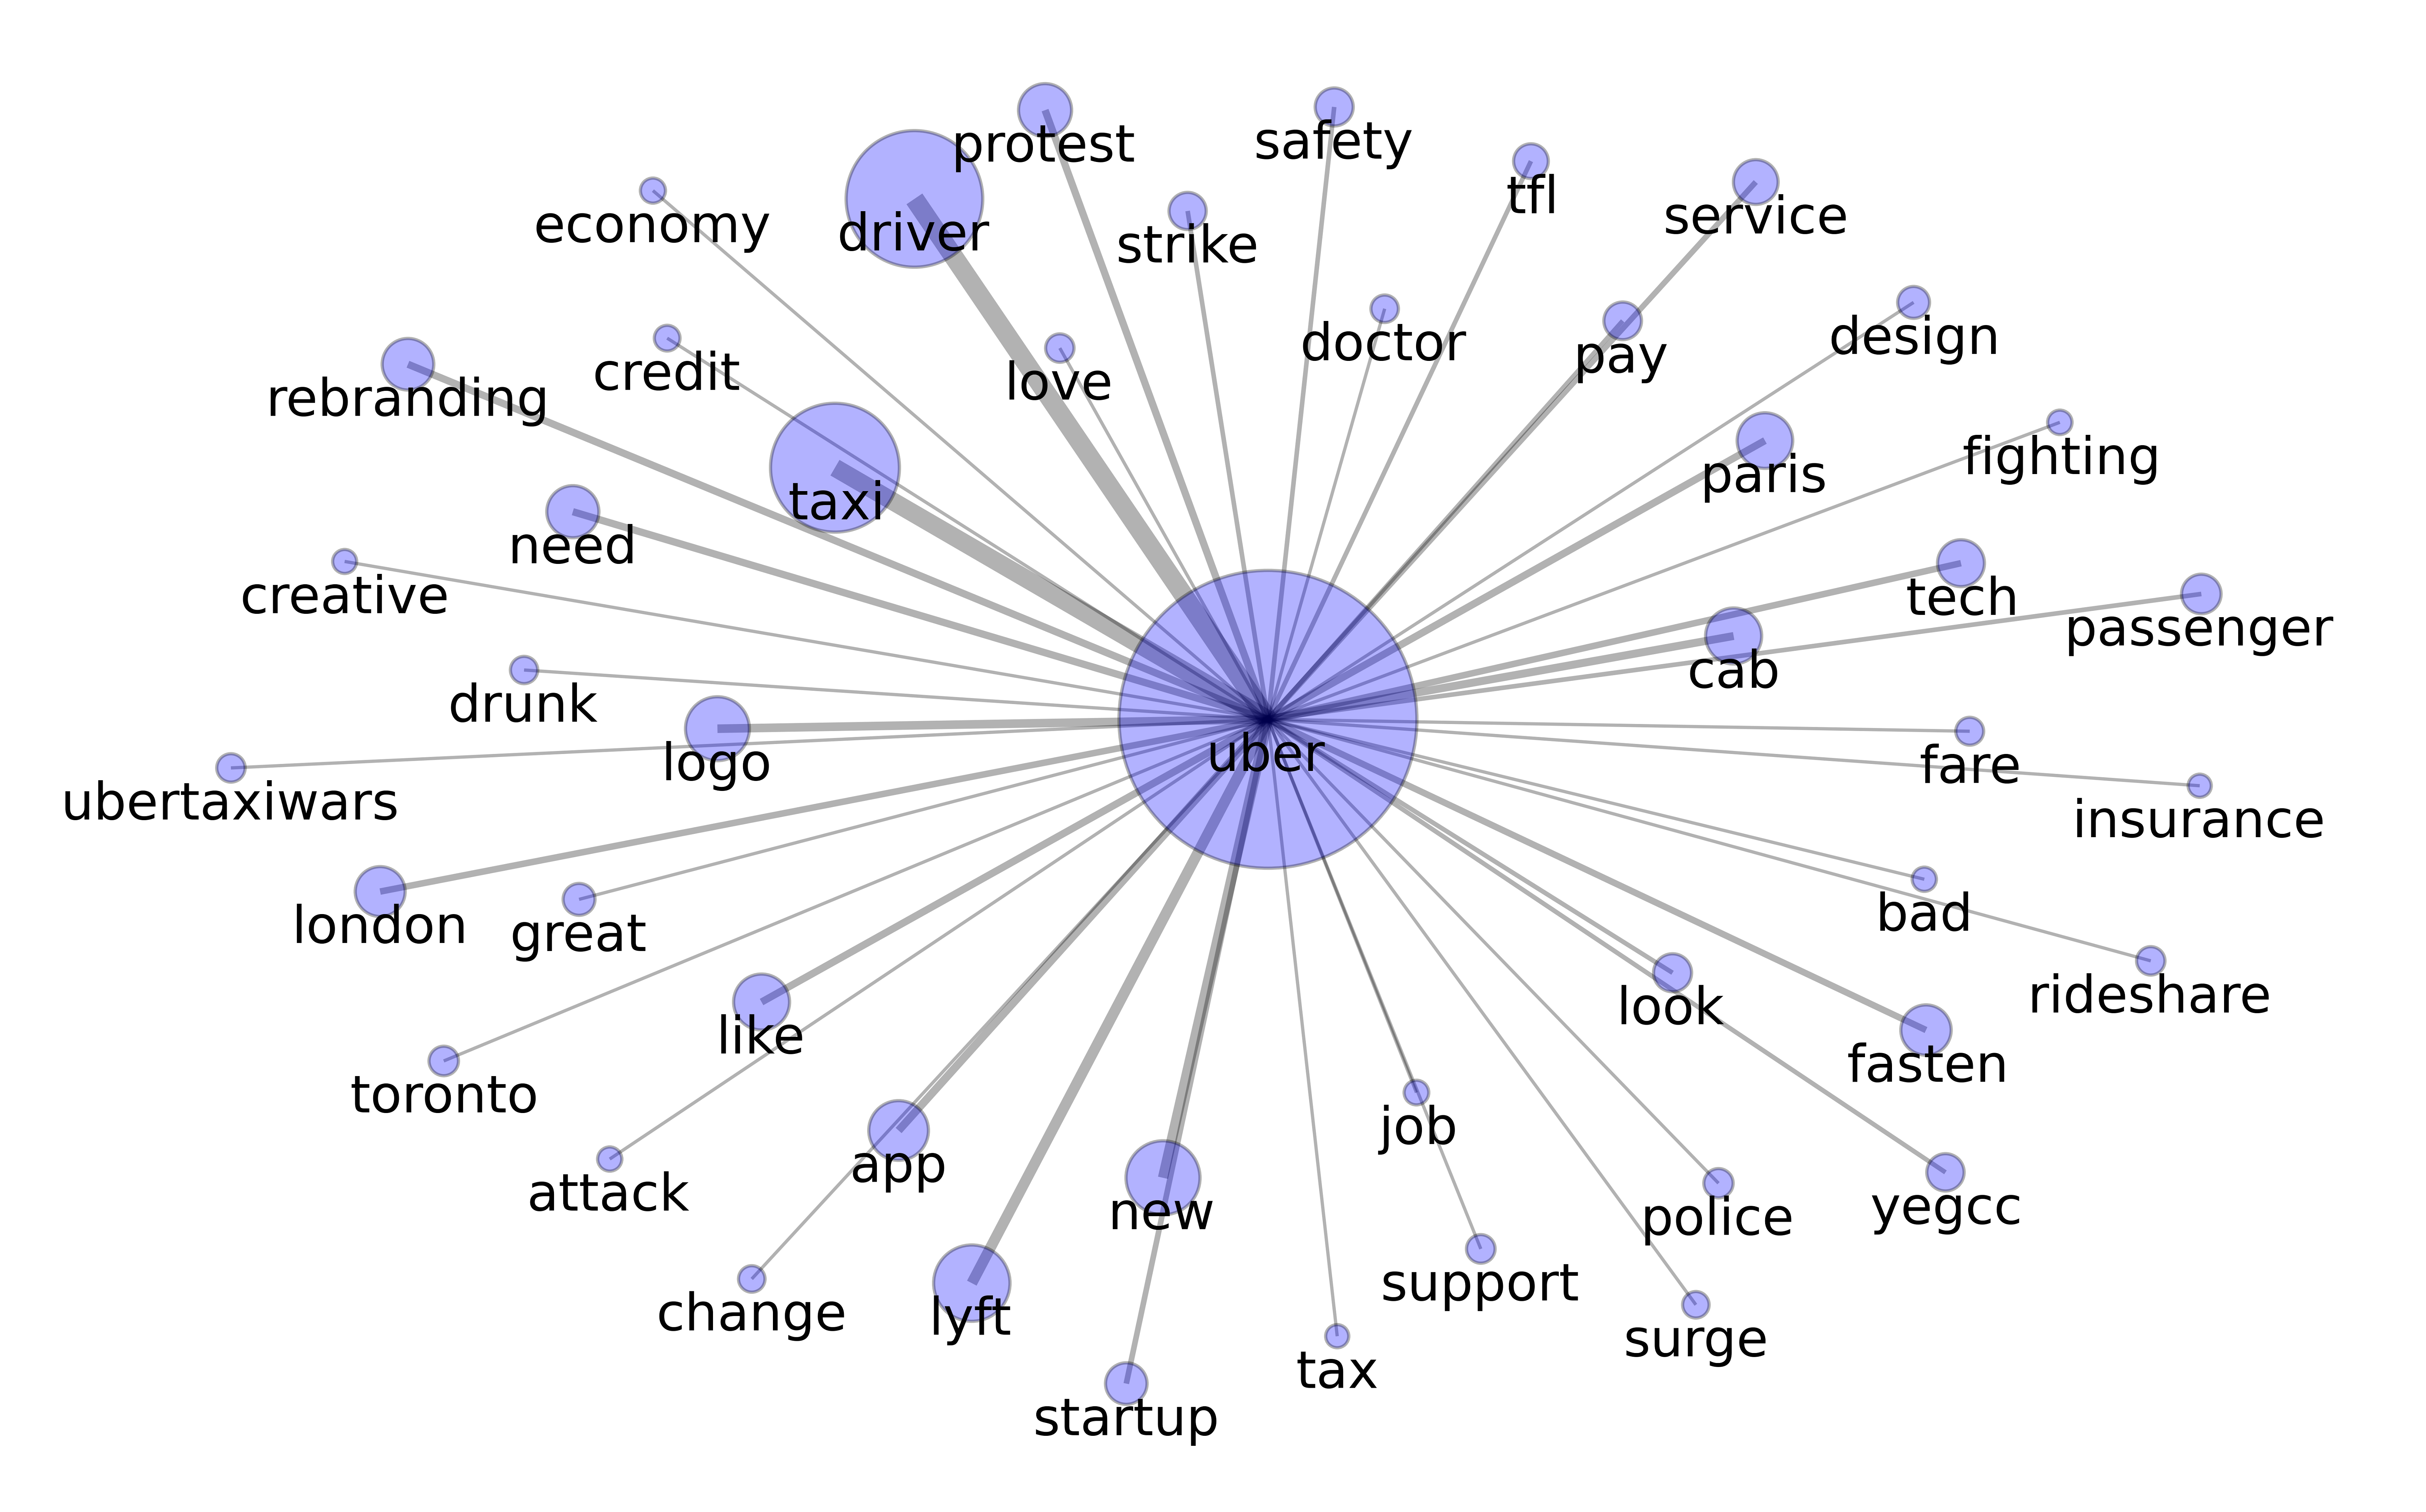
\includegraphics[width=\linewidth]{../figures/Poster_Network.png}
\captionof{figure}{\color{Green} Top Frequency Words Network Graph: Size of the nodes is proportional to their appearing frequencies.}
\end{center}\vspace{1cm} 

\begin{center}
\resizebox{\linewidth}{!}{
\begin{tabular}[2pt]{|r|l|l|l|l|l|l|l|l|l|}
\hline
\multicolumn{10}{|c|}{\cellcolor{blue!25}Top Words Related to Uber} \\
\hline
Top Words & driver & taxi & lyft & new & logo & app & cab & like & protest \\\hline
Frequency & 17828 & 15861  & 5572 & 5237 & 3909   & 3400 & 3009 & 2992 & 2699 \\\hline
\end{tabular}
}

\vspace{0.5 cm}
\small \textbf{Table1}:\color{Green} This table shows the most frequently tweeted words with Uber. 

\color{DarkSlateGray}

\normalsize

\medskip

\begin{tabular}[2pt]{|c|c|}
\hline
% \multicolumn{2}{|c|}{\cellcolor{lightgray}Top Words Related to Uber by Group} \\
\multicolumn{2}{|c|}{\cellcolor{blue!25}Top Words Related to Uber by Group} \\
\hline
Top Topic  & Related words \\\hline
taxi (19645) & taxi, cab, ubertaxiwars \\
logo change (13832) & change, design, logo, look, rebranding, new \\
strike (6978) & paris, protest, strike \\
drunk doctor (2007) & doctor, drunk, attack \\
surge pricing (678) & surge \\\hline
\end{tabular}

\vspace{0.5 cm}

\small \textbf{Table2}:\color{Green} This table gives context to what the most frequently tweeted words with Uber were related to.

\color{DarkSlateGray}
\end{center}
\normalsize
The word "like" is mainly used in a negative context. (Detailed explanation later in the poster.) \\
\newline
From the network diagram and these charts, the top topics related to Uber are \textbf{taxi, logo change, strikes, drunk doctor and surging price}. 

\section*{Where Do People Tweet about Uber in the U.S.?}
%In the section, it is interesting to see varied activeness on twitter about Uber in different states, and they also have their unique concentrations.
\begin{center}\vspace{0cm}
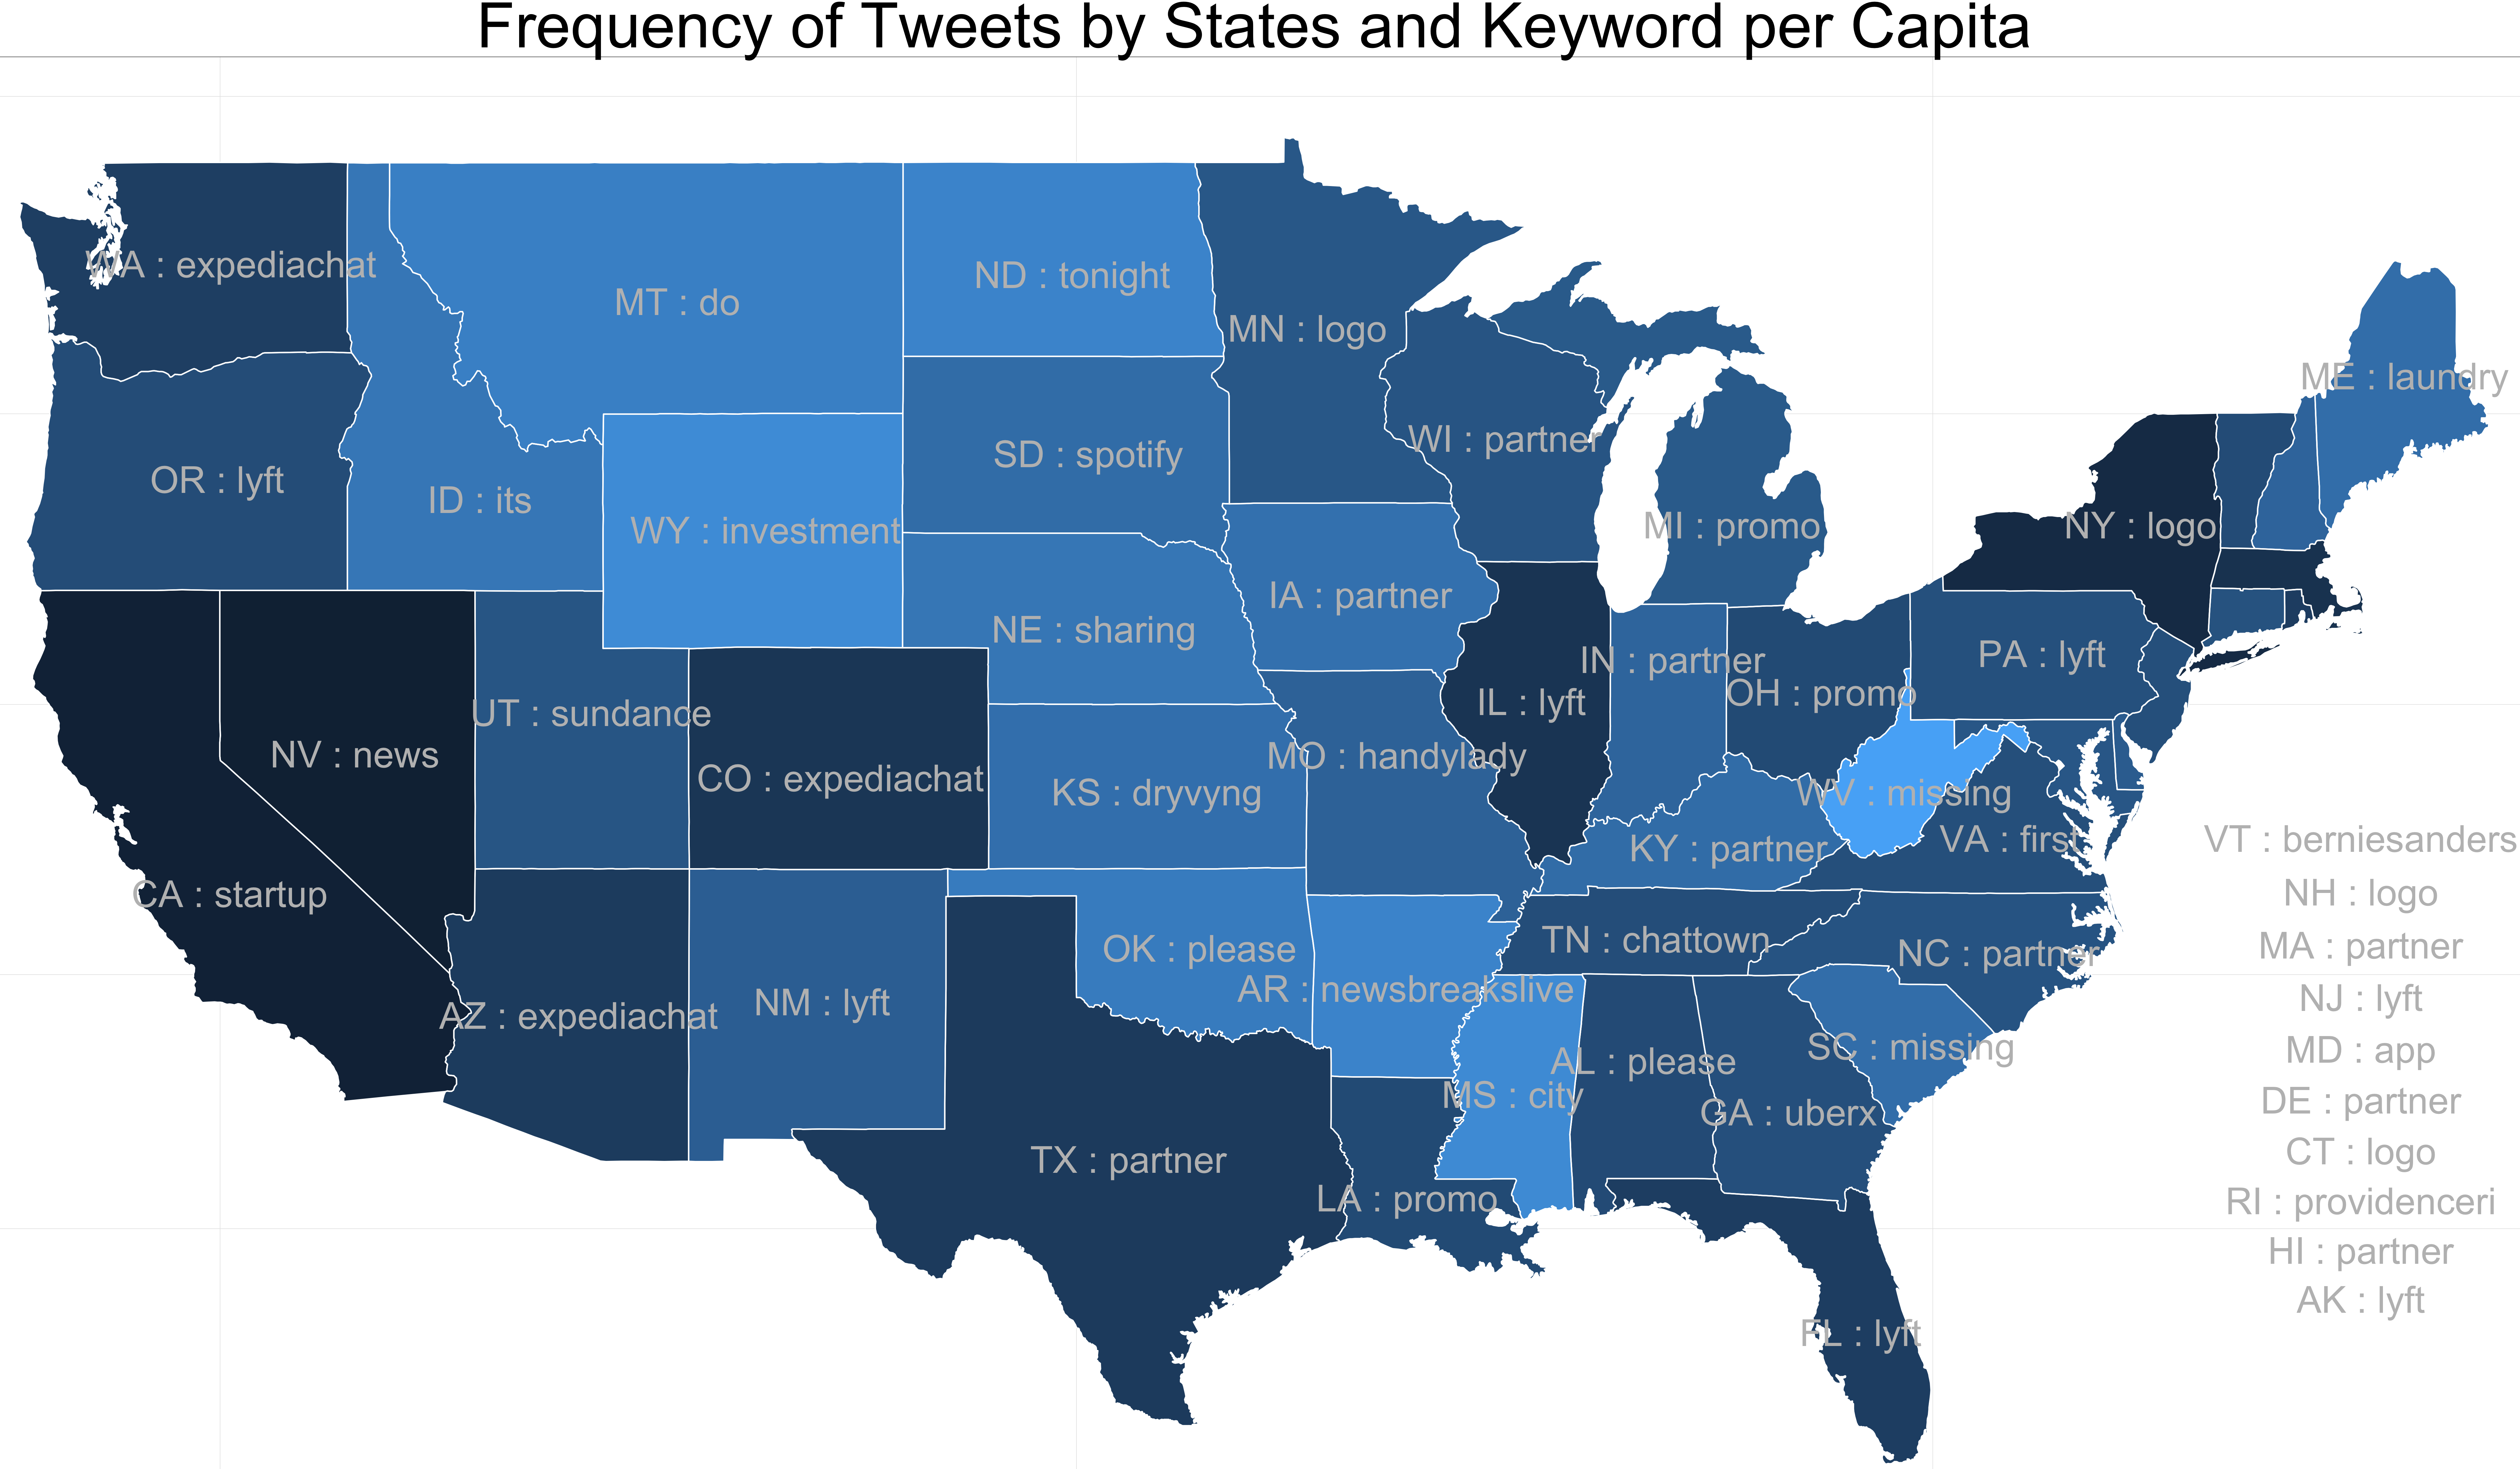
\includegraphics[width=0.9\linewidth, height=5in]{../figures/Poster_Heatmap}
\captionof{figure}{\color{Green} In this heatmap, the darker colored states imply more tweets about Uber. The text in each state is the most frequently tweeted word for the particular state.}
\end{center}\vspace{0cm}
The frequency level in the \textbf{heatmap} is computed from the number of tweets about Uber in each state after normalizing by population. The map shows that California, Nevada and New York are the top three most active states in the U.S.
\\

\begin{center}
\begin{tabular}{|p{2cm}|p{5cm}|p{2cm}||p{2cm}|p{5cm}|p{2cm}|}
    \hline
    \multicolumn{6}{|c|}{\cellcolor{blue!25}Top Used Words by State} \\
    \hline
     State& Keyword&Freq &State& Keyword&Freq\\
     \hline
        CA&startup&965 & NV&news&69\\
	TX&partner&221 & FL&lyft&67\\
	NY&logo&143 & IL&lyft&58\\
	HI&partner&106 &MA&partner&54\\	
	\hline
\end{tabular}
\end{center}
\vspace{0.25 cm} 
\small \textbf{Table 3}: \color{Green} This table shows the most frequently used words in the top 10 most active states. The U.S. data is a subset of the larger global dataset.
\normalsize
\color{DarkSlateGray}

\begin{itemize}
  \item \textbf{startup}: Californians love to talk about startups with Uber, as Uber is one of the fastest growing up startups worldwide.
  \item \textbf{logo}: New Yorkers seems to be very passionate about new Uber logo.
  \item \textbf{Lyft}: People in Florida and Illinois tend to juxtapose Lyft and Uber, as these companies have similar business and  are very active in both states.
  \item \textbf{partner}: Uber has an expanding business in Texas and Massachusetts, resulting in a lot of advertisements about ``how to be a Uber \textbf{partner}''. ``Uber partner'' has the same meaning as ``Uber driver'' 
\end{itemize}

\section*{Negative Tweets About Uber}
\begin{center}\vspace{1cm}

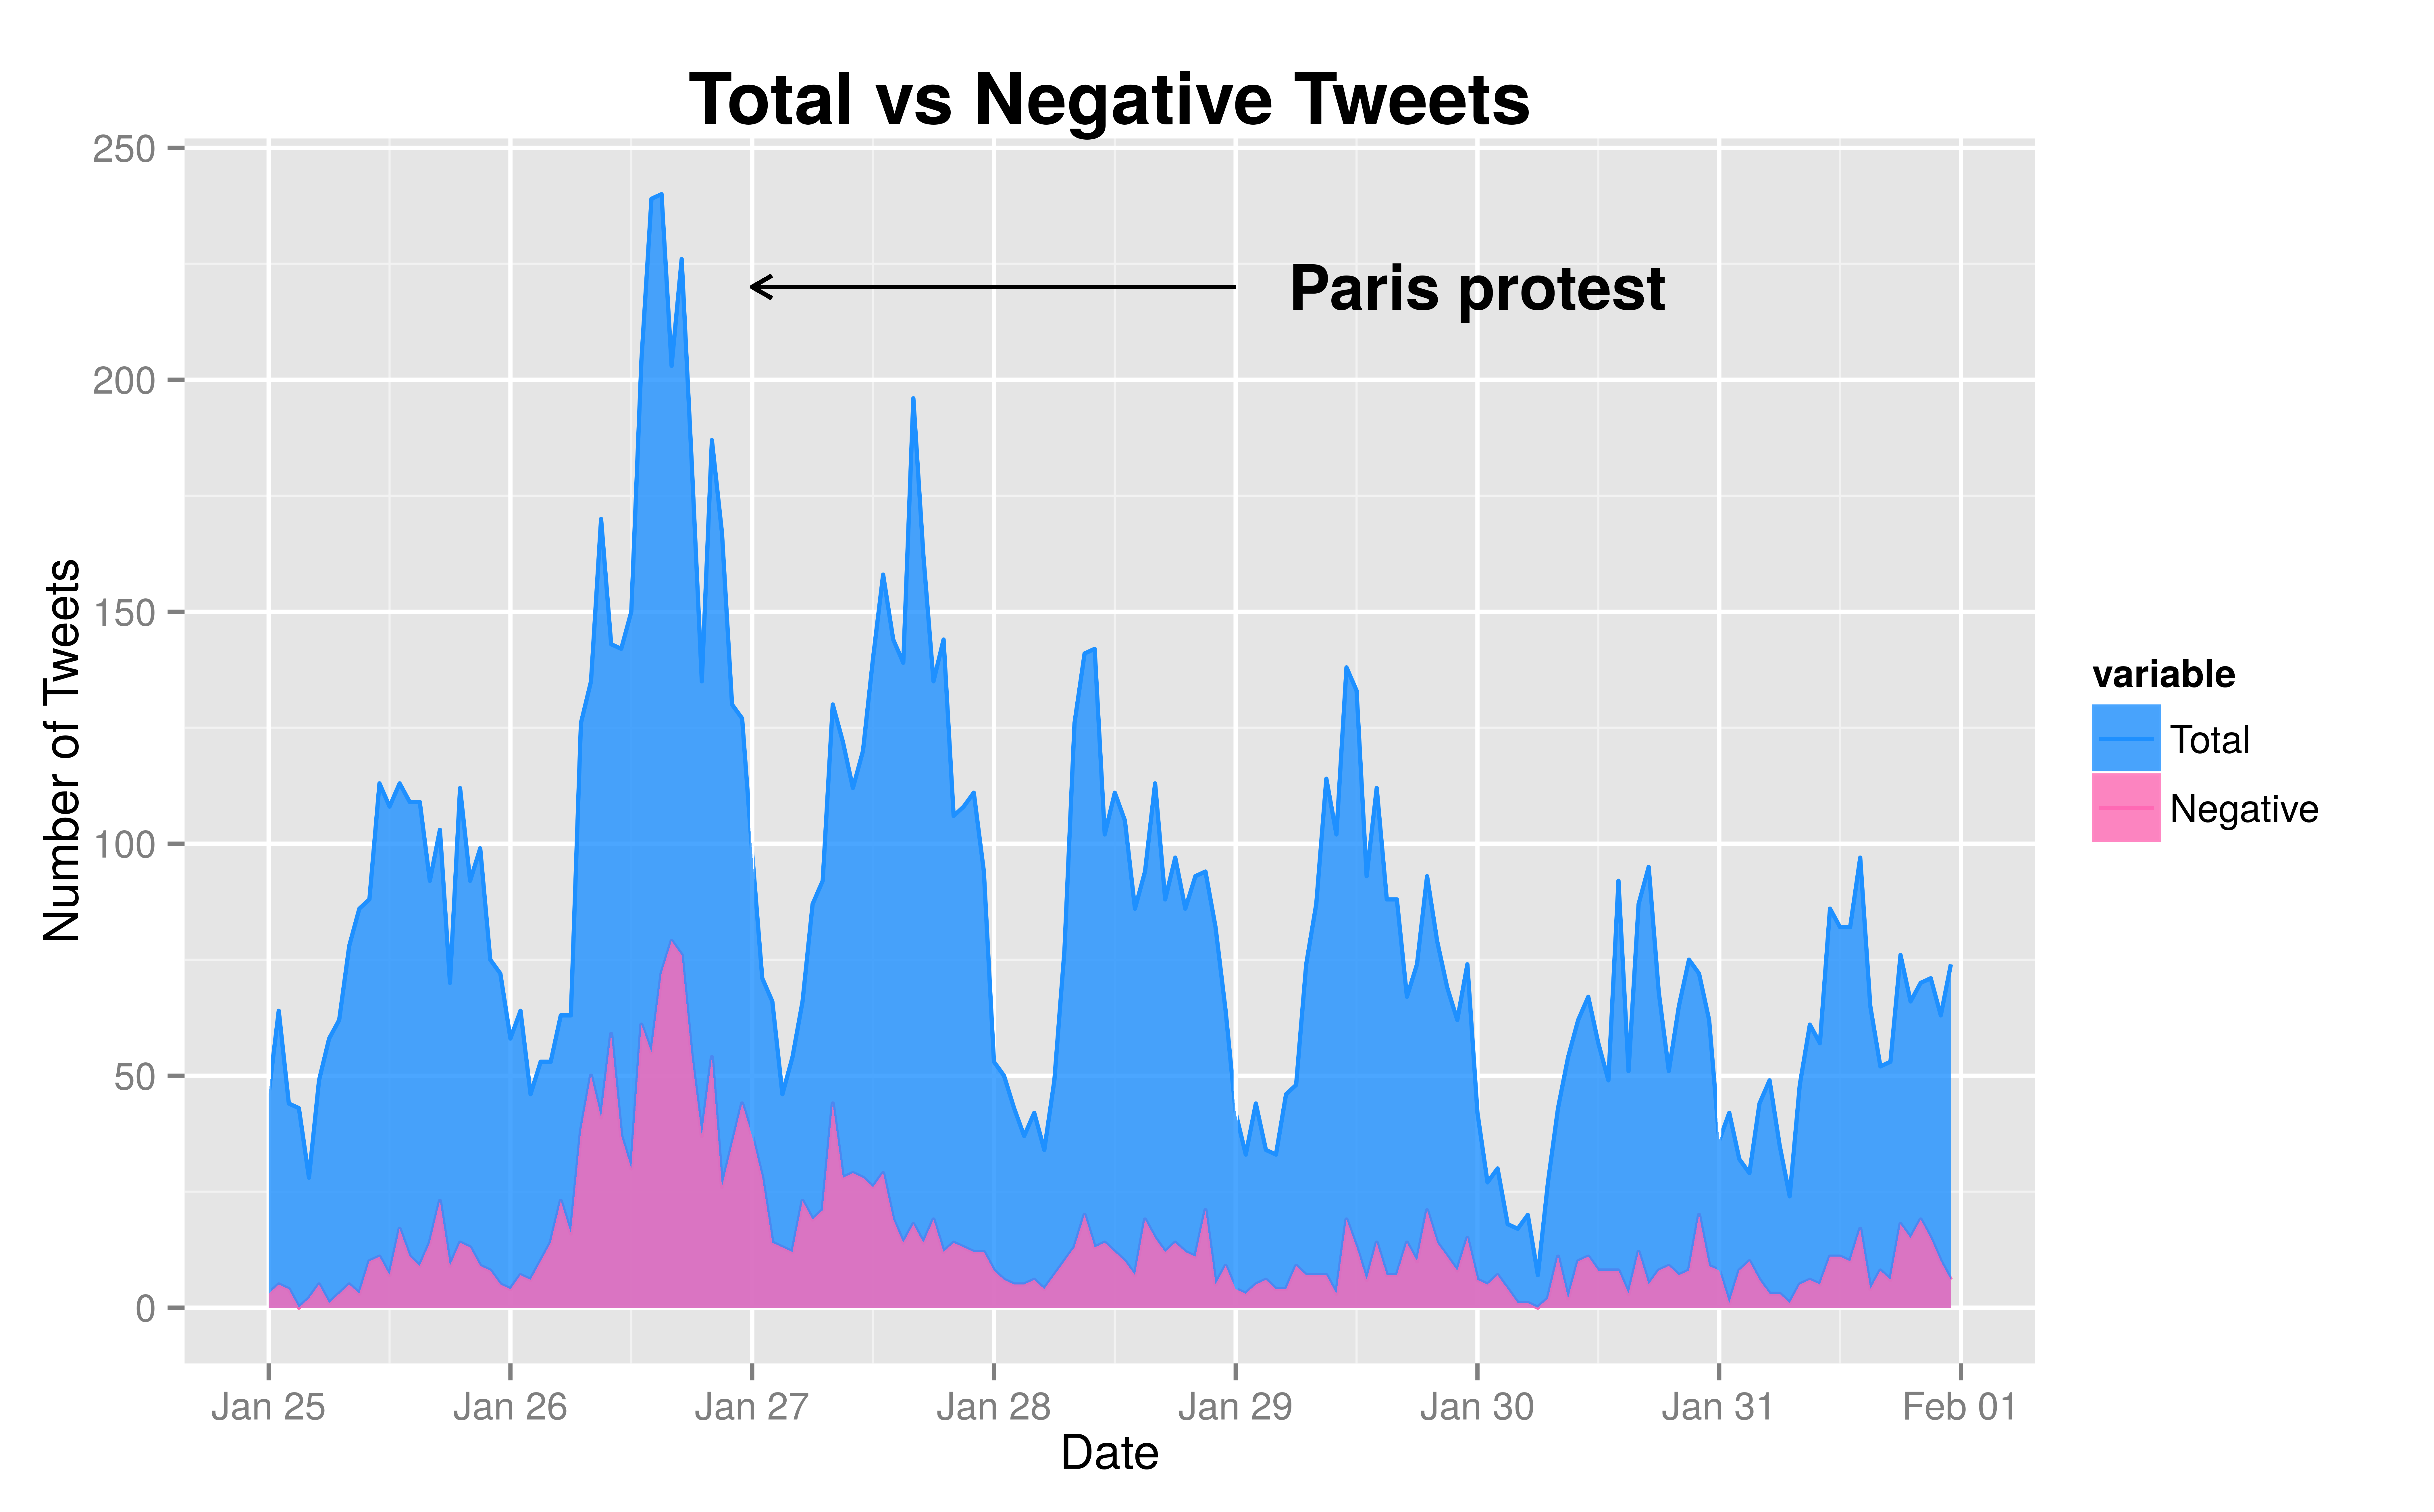
\includegraphics[width=\linewidth, height=5in]{../figures/Poster_TotalNegTweets.png}
\captionof{figure}{\color{Green} This is a one-week time series plot, presenting the time and the amount people tweet about Uber. The proportion of negative tweets is depicted in pink.}

\end{center}\vspace{0.25 cm}

In general, people tweet less about Uber on weekends. Most tweets happen around rush hour or party times. \\
The amount of negative tweets is generally proportional to the amount of total tweets.

\begin{center}\vspace{0.5 cm}

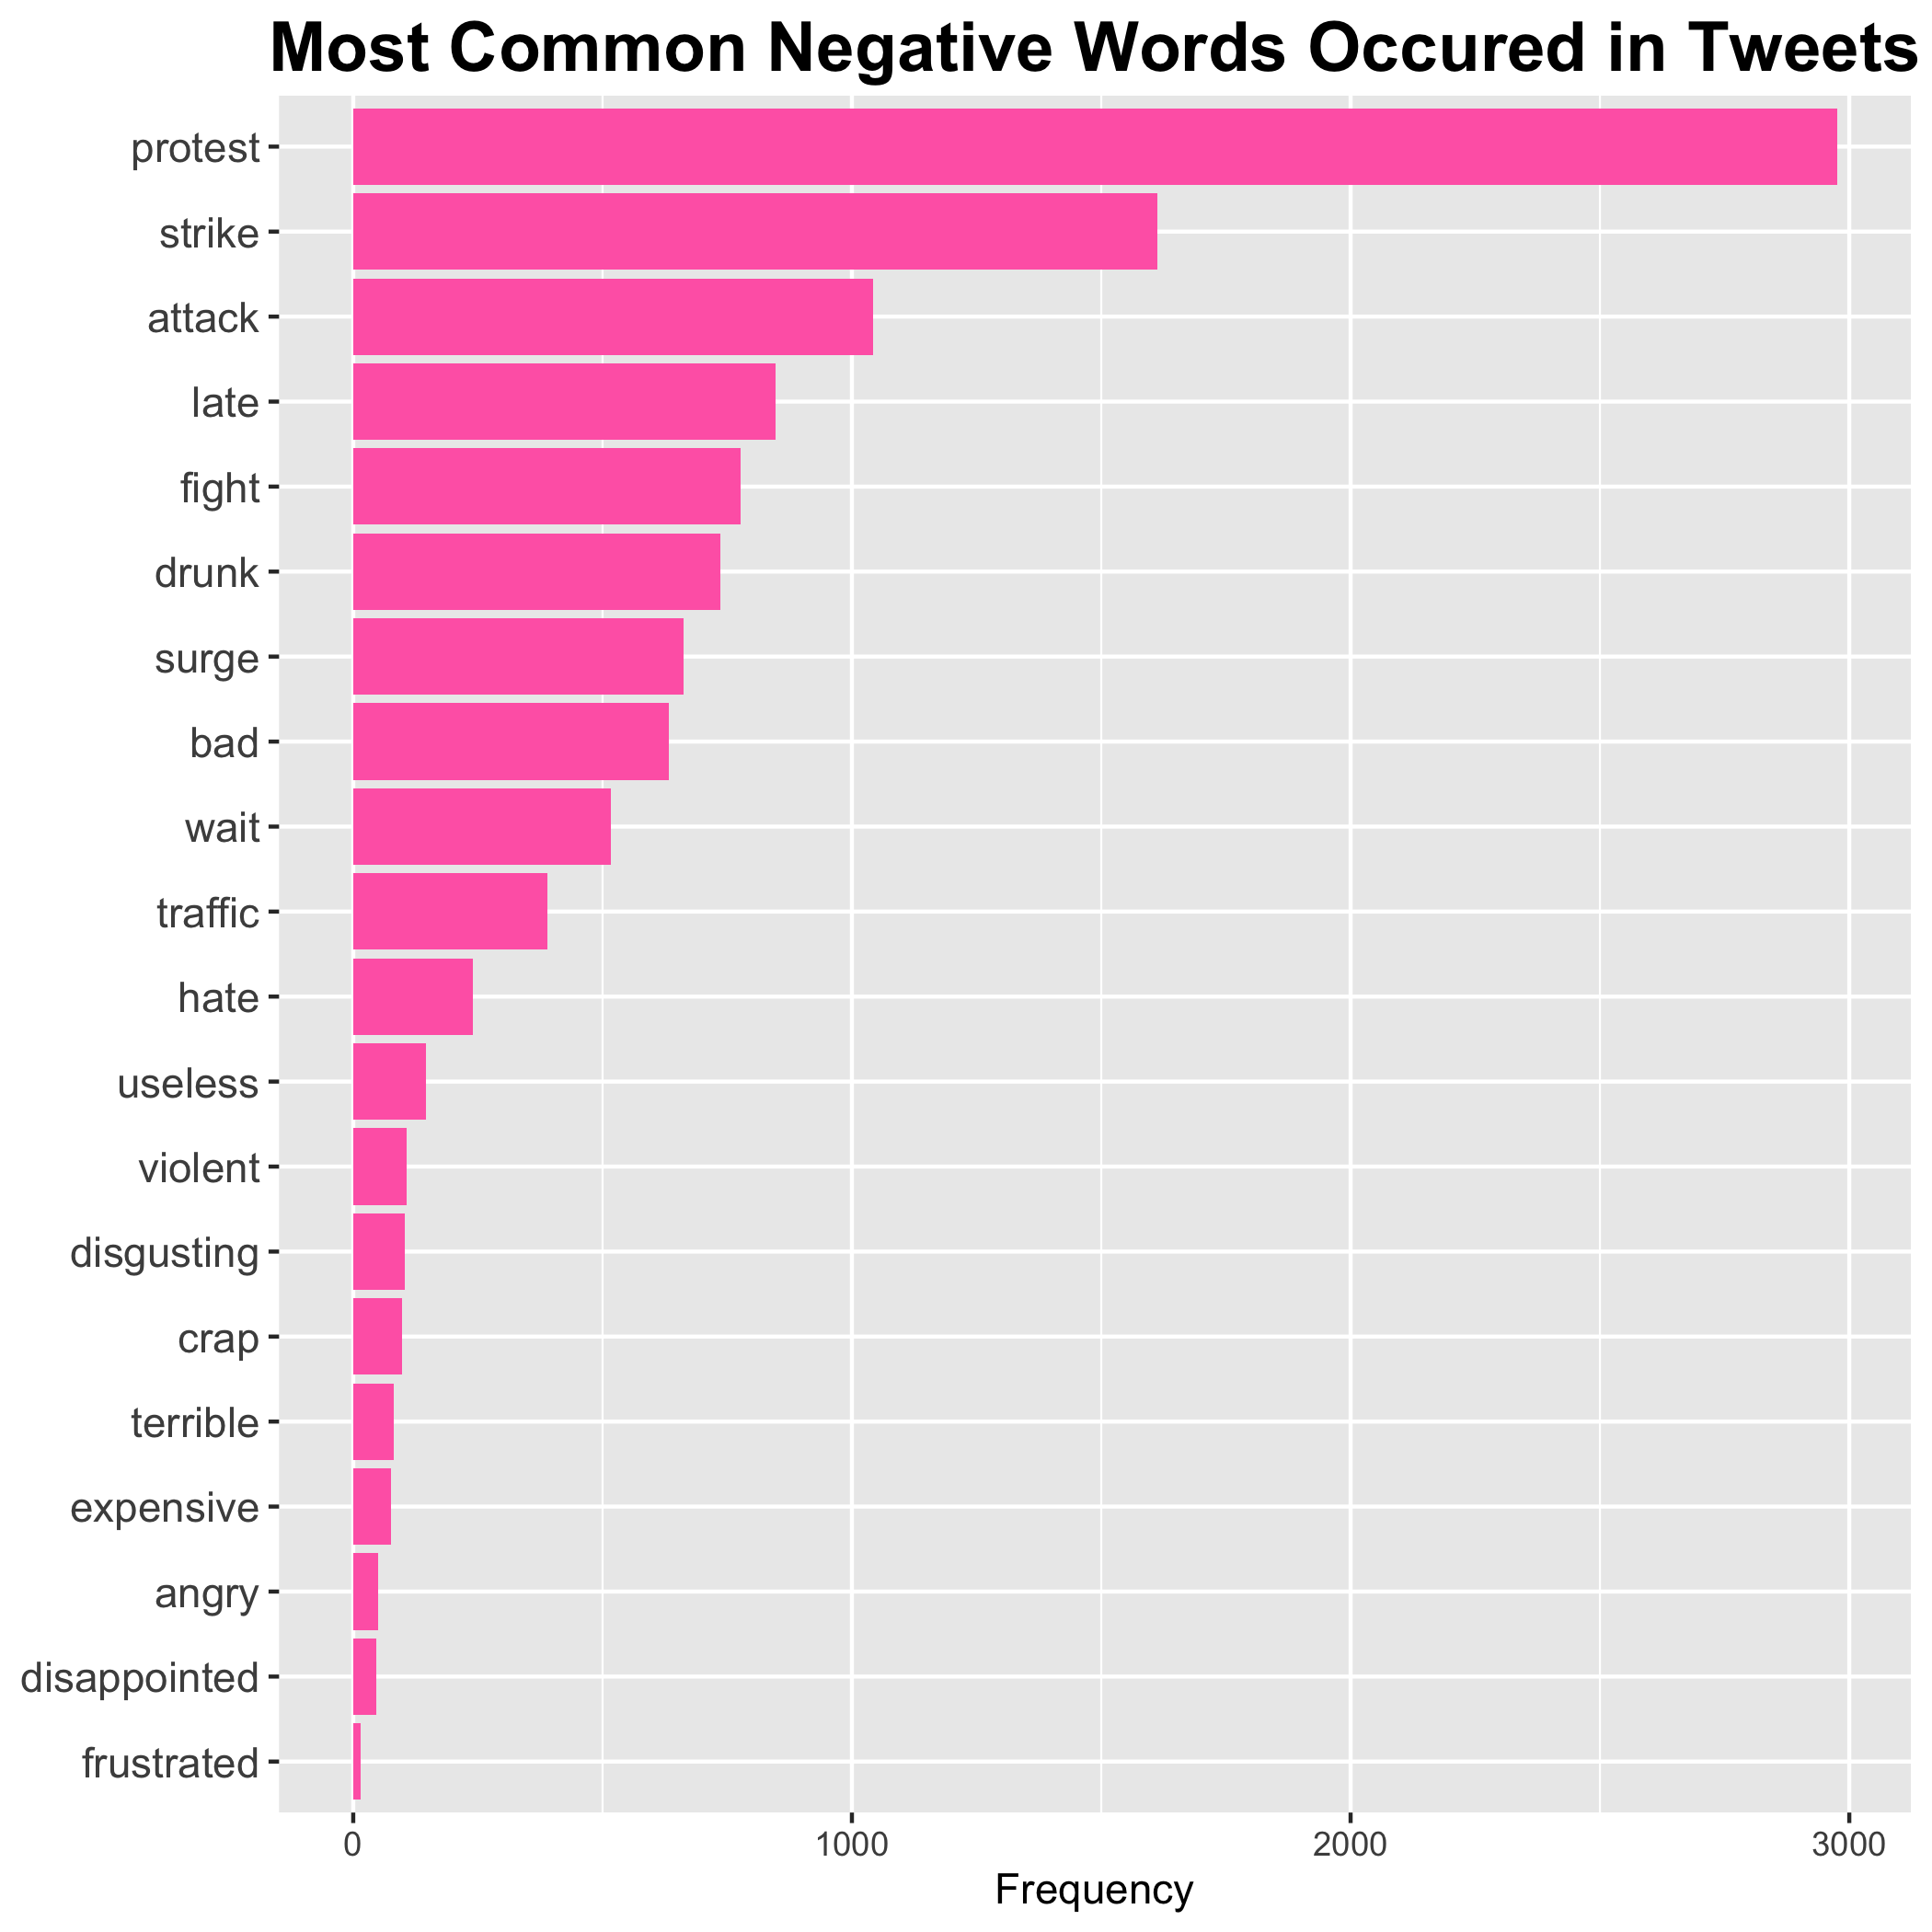
\includegraphics[width=\linewidth, height=5in]{../figures/Poster_NegWords.png}
\captionof{figure}{\color{Green} This shows the most common negative words occurred in tweets. X-axis represents the true value of frequency. As shown above, Protest and strike has significant high frequency. }

\end{center}\vspace{0.25 cm}

\section*{When does Surge Pricing Occur?}
\begin{center}\vspace{1cm}

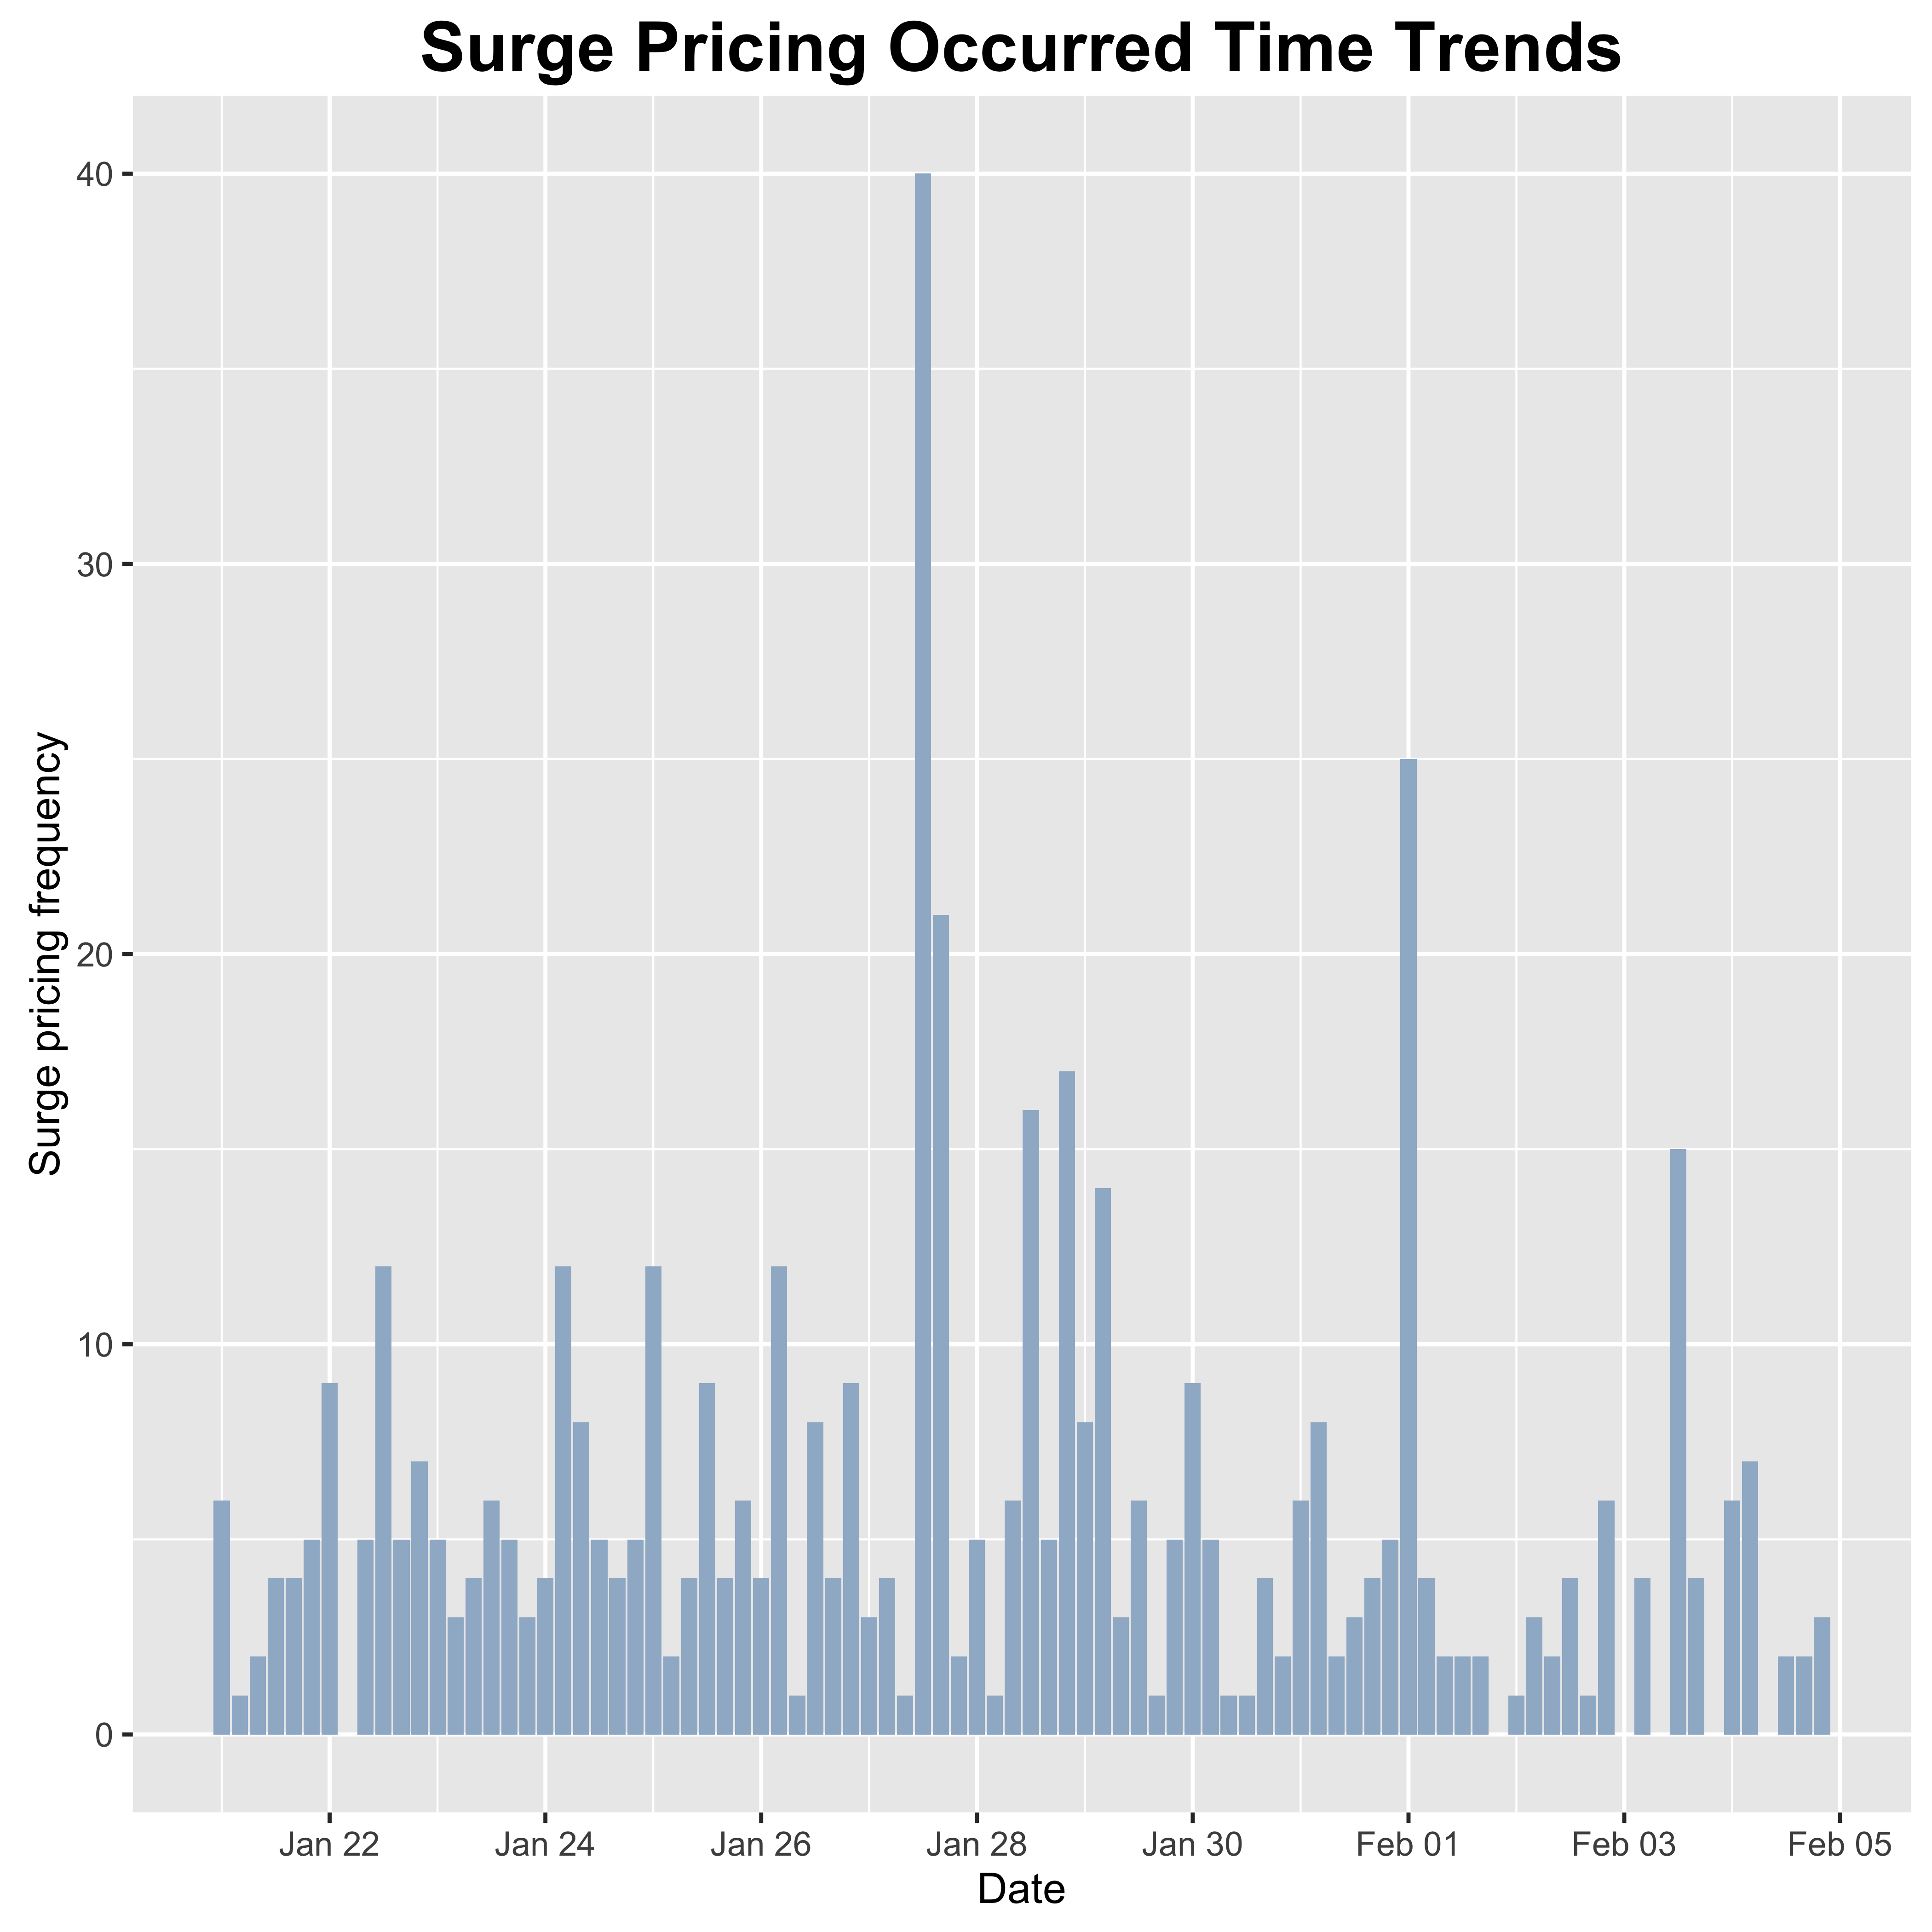
\includegraphics[width=\linewidth, height=5in]{../figures/Poster_TimeSeries.png}
\captionof{figure}{\color{Green} This is time-series plot for two weeks from Jan 21st to Feb 4th. Each bar represents a 4-hour period. It shows the frequency of surge pricing occurred per bin.}

\end{center}\vspace{0.25 cm}

Although there are certain spikes in the surge-pricing, we do not see any discernible patterns. We further explore the patterns of surge-pricing in the the following plot.

\begin{center}\vspace{0.75 cm}

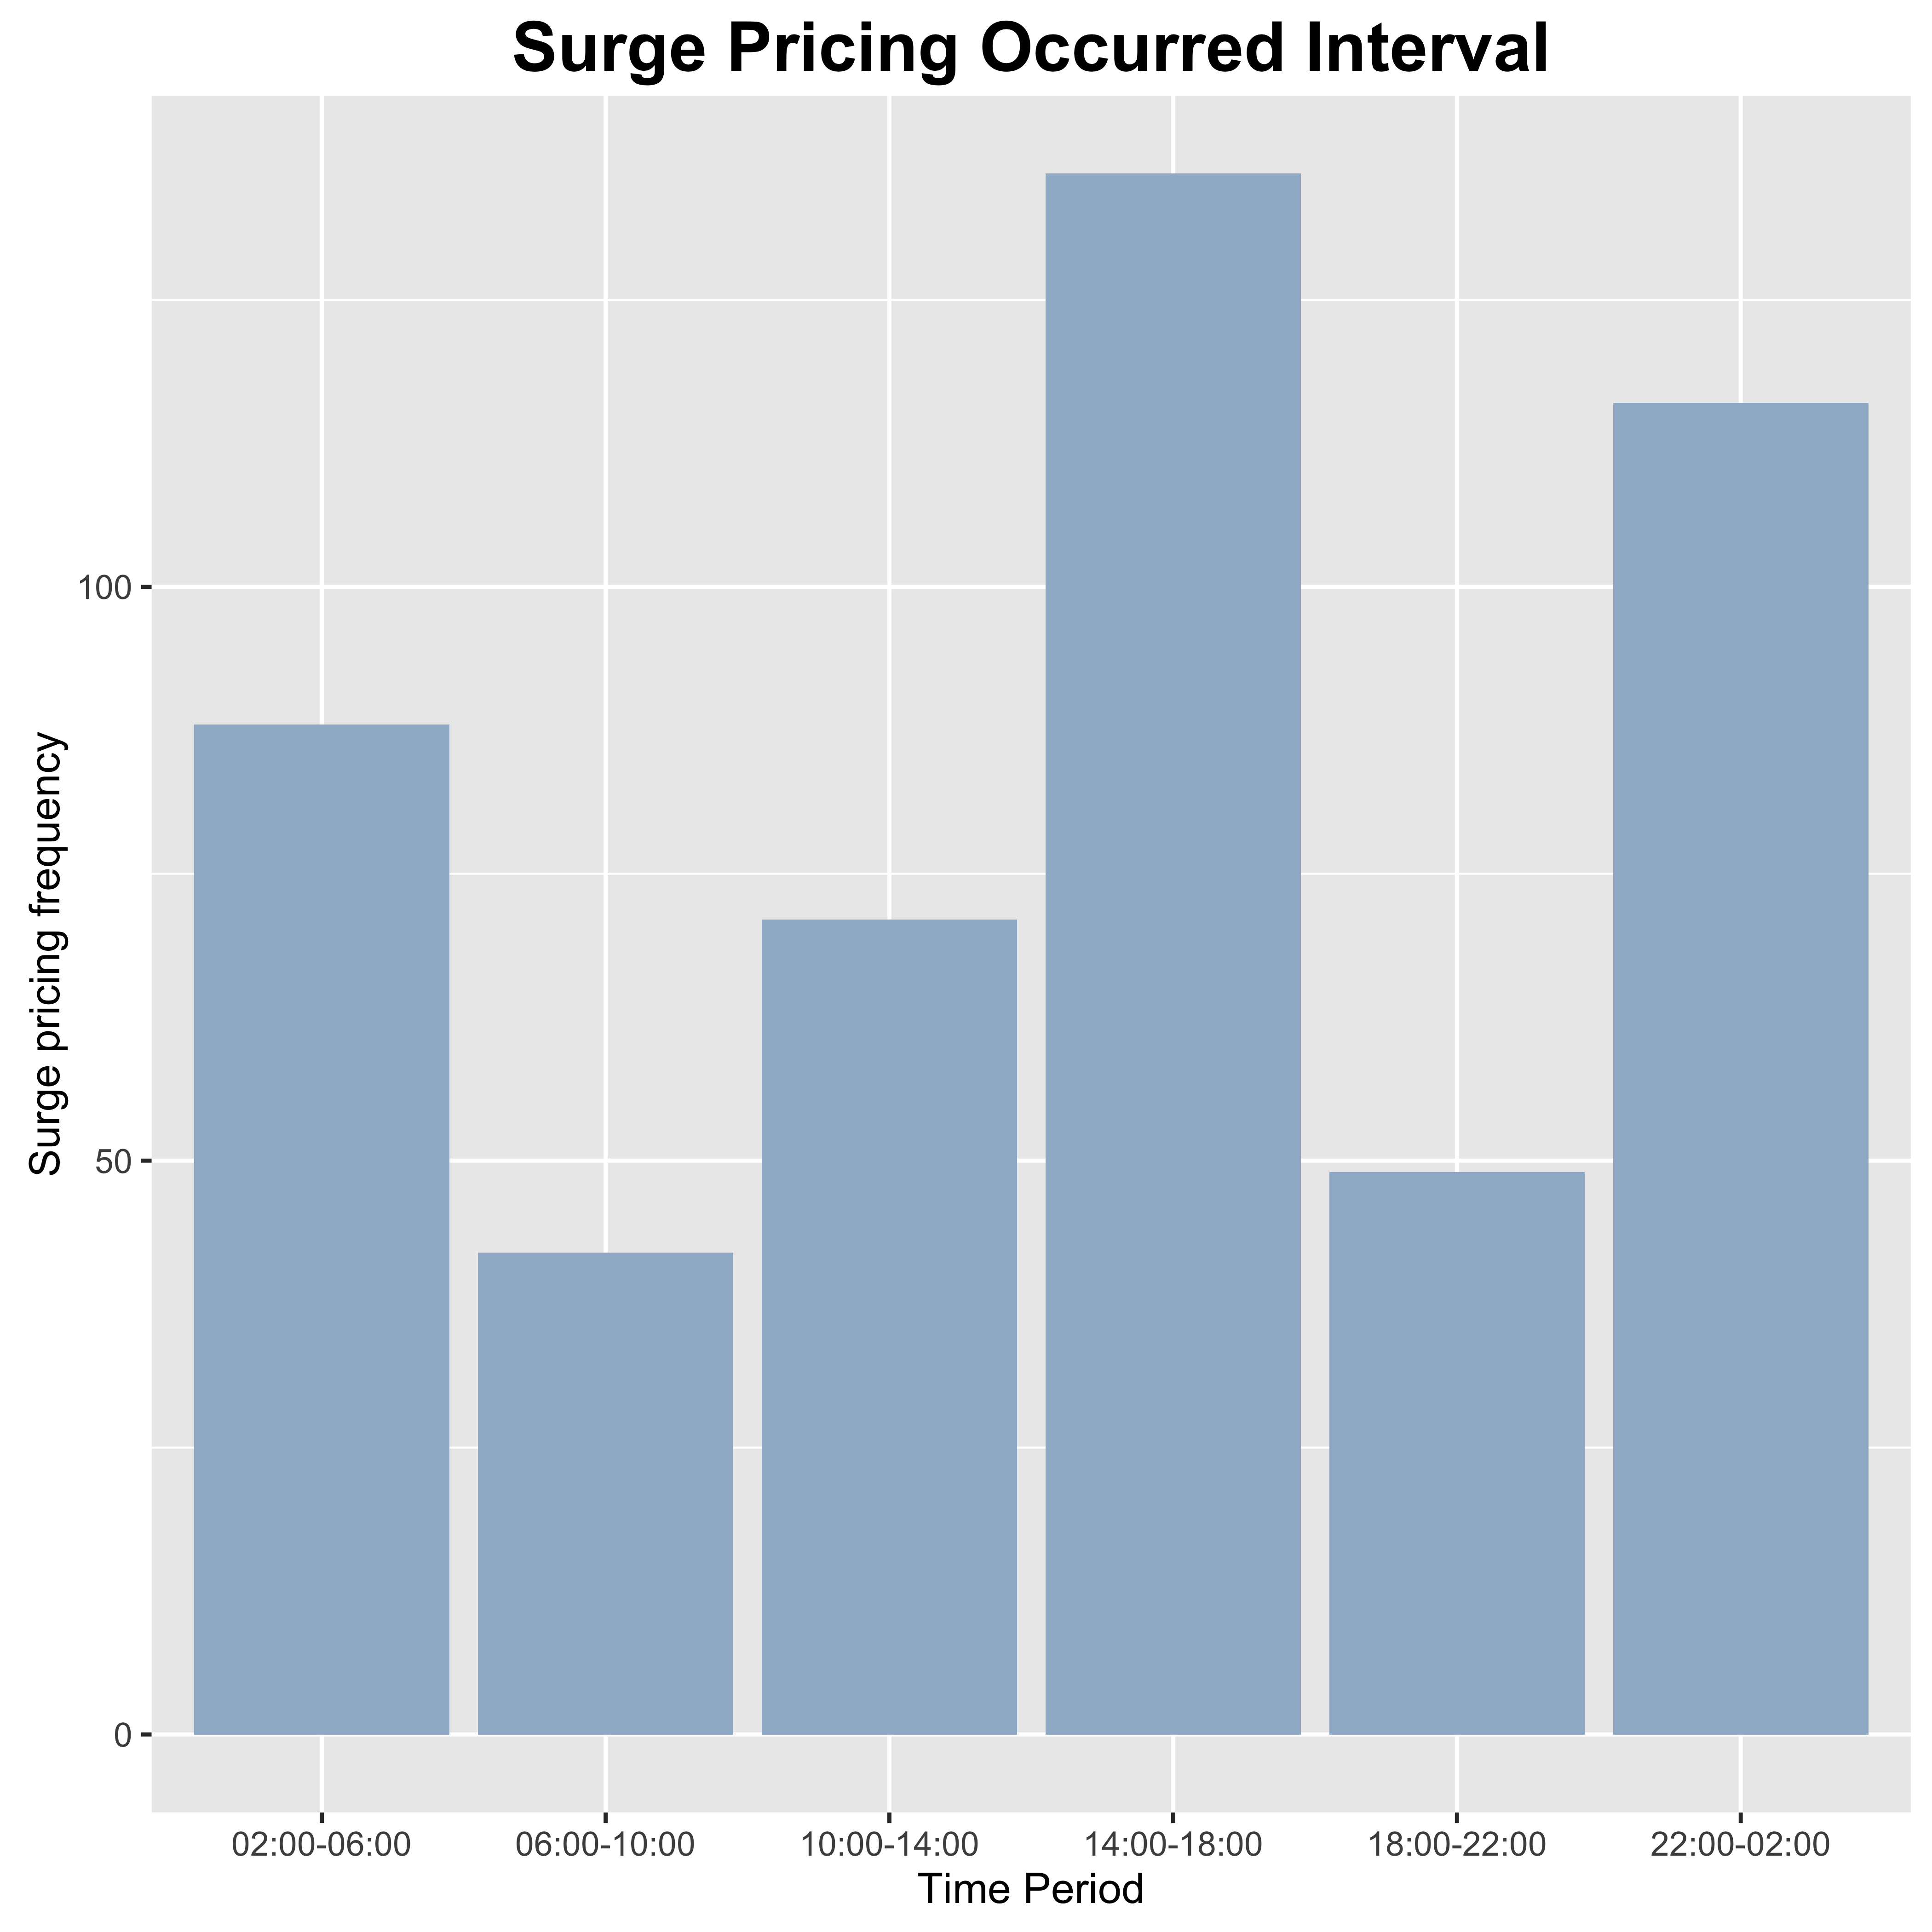
\includegraphics[width=\linewidth, height=5in]{../figures/Poster_SurgeGroup.png}
\captionof{figure}{\color{Green} Each bar in this plot represents the frequency of surge-pricing occurring in each 4-hour period. The frequency is calculated based on the previous plot by summing all the same four-hour periods in two weeks together. It indicates that surge pricing tends to occur during 14:00-18:00 (rush hour) and 22:00-2:00 (party times).}

\end{center}\vspace{0.25 cm}

\section*{Uber Changes Its Logo}
\vspace{0.25 cm} 

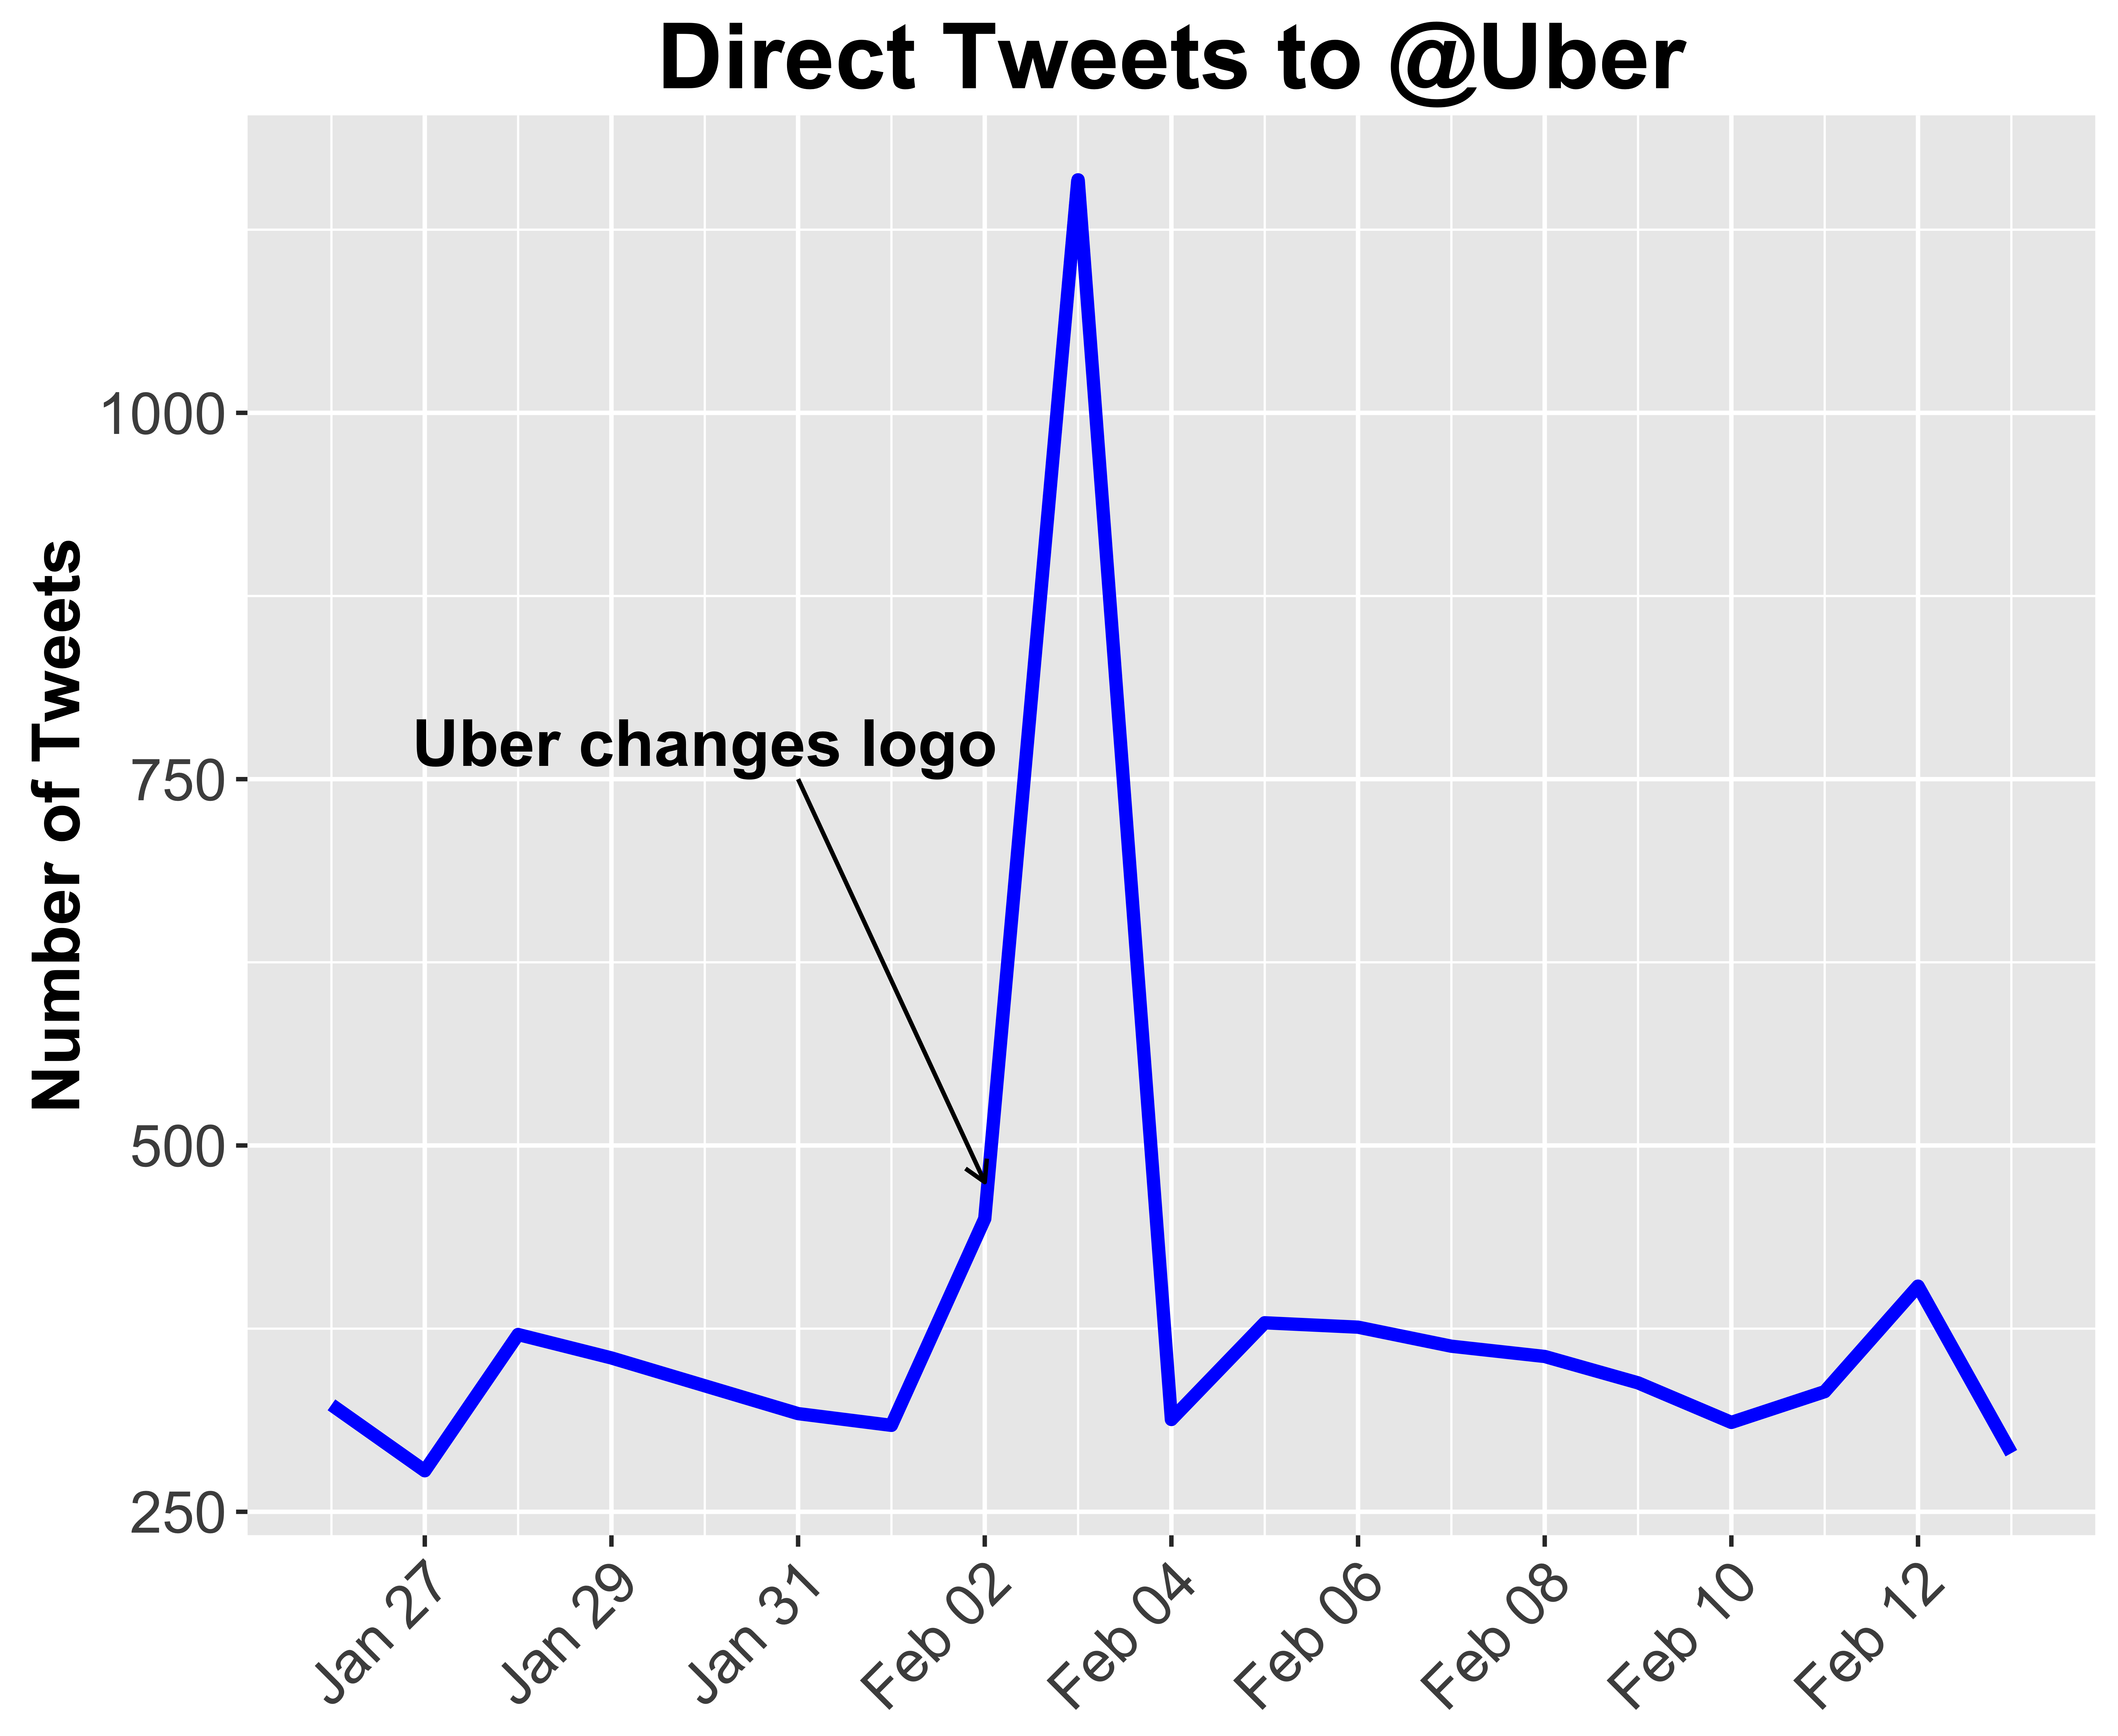
\includegraphics[width=\linewidth, height=5in]{../figures/Poster_LogoAnnounce.png}
\captionof{figure}{\color{Green} Upon announcement of Uber's new logo on February 2nd, 2016, the number of tweets directed to @Uber rose dramatically.}
 
\begin{center}
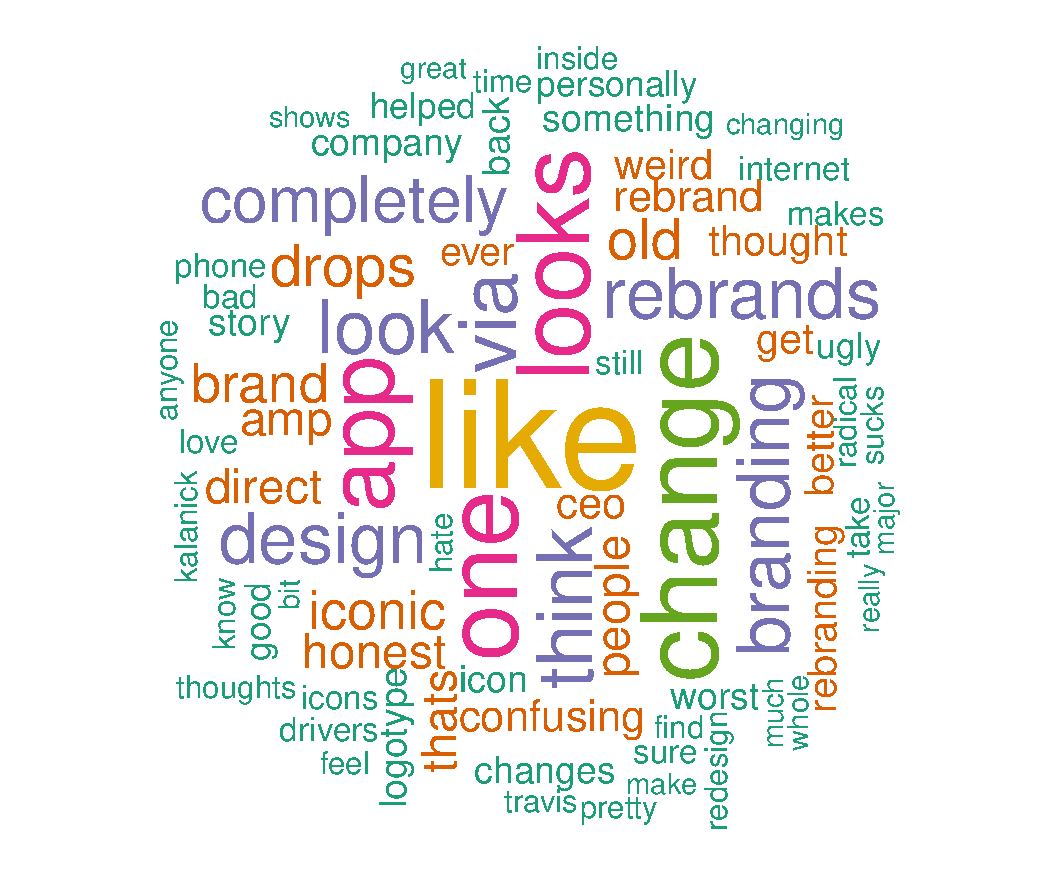
\includegraphics[width = .7\linewidth, height = 15 cm]{../figures/Poster_WordCloudLogo.pdf}
\captionof{figure}{\color{Green} Most used word is 'like'.}
\hfill
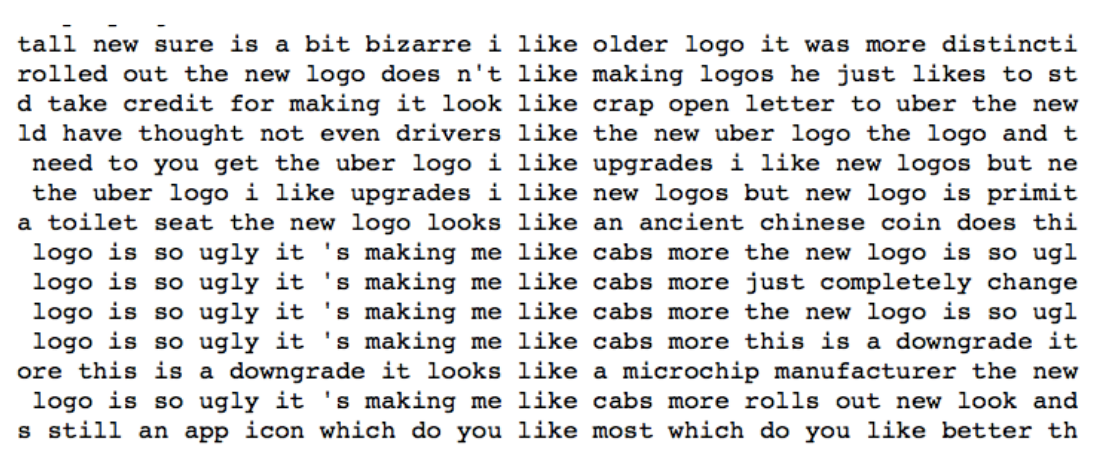
\includegraphics[width = \linewidth, height = 10 cm]{../figures/Poster_LogoLike.png} 
\end{center}

The most frequently used word in tweets pertaining to the logo change was 'like', as shown above. Contrary to intuition, 'like' was used in a negative context most of the time, as evidenced by the sample tweets above.

\color{DarkRed}

\section*{Conclusions}
\begin{itemize}
\item California, New York, and Nevada have the most tweets per person
\item The most frequent negative keywords are protest, strike, and attack. These are driven by Paris Uber protest
\item Negative tweets represent a larger proportion of total tweets in periods of spikes based on our data
\item The public had a generally negative but short-term reaction to Uber's new logo
\end{itemize}


\color{DarkSlateGray} % Set the color back to DarkSlateGray for the rest of the content

%----------------------------------------------------------------------------------------
%	FORTHCOMING RESEARCH
%----------------------------------------------------------------------------------------

% \section*{Potential future steps}
% \begin{itemize}
% \item Analyze the correlation and time-series pattern among uber real-time usage, surge pricing level
% \item Marketing 
% \end{itemize}

% The correlation and time-series pattern among uber real-time usage, surge pricing level and the number and content of tweets will be very interesting to look at. Another interesting question related to marketing strategy and network mechanism is: is it better to release marketing tweets with promotion code or free rides when some event triggers large spike of negative tweets? Or is it better to release it during quiet period? We are not able to study these questions because we don’t have user’s data and we cannot conduct experiment on marketing tweets. However, we may well work for Uber in the future to finish these steps and lots more!



 %----------------------------------------------------------------------------------------
%	REFERENCES
%----------------------------------------------------------------------------------------

% \nocite{*} % Print all references regardless of whether they were % cited in the poster or not
% \bibliographystyle{plain} % Plain referencing style
% \bibliography{sample} % Use the example bibliography file % sample.bib

%----------------------------------------------------------------------------------------
%	ACKNOWLEDGEMENTS
%----------------------------------------------------------------------------------------


\end{multicols}
\end{document}